\section{Interface}

Nesta secção é explicada a interface da aplicação, ou seja, o \textit{flow} entre as várias janelas, assim como o que o utilizador pode fazer nestas e a forma para tal.

\subsection{Login}
Iniciando a aplicação, o utilizador fica perante a janela de \textit{login}, apresentada na Figura \ref{loginframe}. 
\begin{figure}[H]
	\centering
	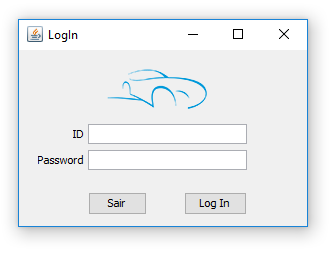
\includegraphics[]{loginframe.png}
	\caption{Login Frame}
	\label{loginframe}
\end{figure}

Para o efetuar, é necessário, antes de tudo, estar registado no sistema e, para tal, apenas o administrador (com conta predefinida) o poderá fazer.

Nesta janela, e conforme o tipo de funcionário que esteja a realizar o login, a próxima janela é uma das seguintes:
\begin{itemize}
	\item Stand (ver Secção \ref{standsec})
	\item Fábrica (ver Secção \ref{fabricasec})
	\item Gestão de funcionários (ver Secção \ref{adminsec})
\end{itemize}

\subsection{Stand}
\label{standsec}

Iniciando sessão como \textit{Funcionário de loja}, a janela correspondente é a apresentada na Figura \ref{standframe}.
\begin{figure}[H]
	\centering
	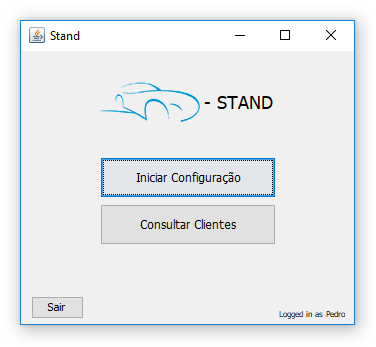
\includegraphics[]{standframe.png}
	\caption{Stand Frame}
	\label{standframe}
\end{figure}

A partir daqui o utilizador pode iniciar uma configuração, consultar todos os clientes registados no sistema ou fazer \textit{logout} através dos botões \textit{"Iniciar Configuração"}, \textit{"Consultar Clientes"} e \textit{"Sair"}, respetivamente. Nesta janela, é também possível ver o utilizador que está com sessão iniciada no canto inferior direito.

\subsubsection{Configuração}
Na criação de uma configuração podem ser adicionadas componentes ou pacotes de componentes.

\begin{figure}[H]
	\centering
	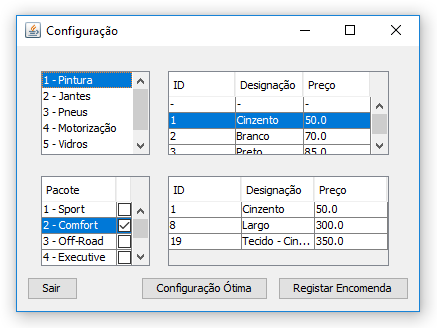
\includegraphics[]{configframe.png}
	\caption{Configuração Frame}
	\label{configframe}
\end{figure}

Para adicionar uma componente é preciso, primeiro, escolher o seu tipo e, só depois, é que se torna possível selecioná-la. Para a escolha de um pacote, é possível visualizar o seu conteúdo primeiro clicando no pacote desejado. O pacote apenas fica selecionado quando é feito \textit{double click} sobre o mesmo (aparecendo um visto no pacote). Tal comportamento pode ser visualizado na Figura \ref{configframe}.
Neste processo de adicionar componentes podem surgir casos em que a componente desejada cria incompatibilidades com uma ou mais componentes já existentes na configuração ou, então, a componente a adicionar ter componentes que são complementares e necessitam também de ser adicionadas. A resolução destes problemas é resolvida conforme as figuras abaixo:

\begin{figure}[H]
	\centering
	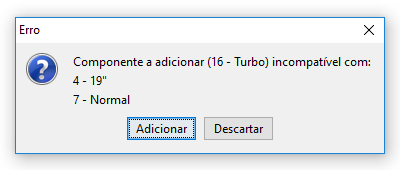
\includegraphics[]{incompativeis.png}
\end{figure}

\begin{figure}[H]
	\centering
	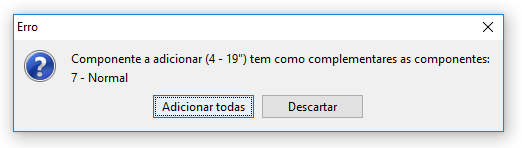
\includegraphics[]{complementares.png}
\end{figure}




\myparagraph{Encomenda}

Neste janela (Figura \ref{regencomendaframe}), é possível para o funcionário selecionar o cliente que está a realizar a configuração, assim como verificar todas as componentes presentes na configuração, o total do preço individual das componentes, o desconto total originado pelos pacotes e o preço final da encomenda. Caso o cliente não exista no sistema, é ainda possível criá-lo a partir desta janela (processo de criação explicado na Secção \ref{novocliente}). Após selecionar o cliente e verificar as componentes, é necessário registar a encomenda clicando em \textit{Registar Encomenda}.

\begin{figure}[H]
	\centering
	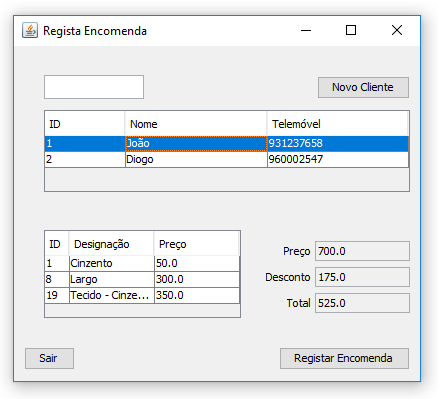
\includegraphics[]{regencomendaframe.png}
	\caption{Encomenda Frame}
	\label{regencomendaframe}
\end{figure}

Caso o funcionário não selecione um cliente ou clique no botão \textit{"Sair"}, são mostradas as seguintes mensagens de erro, respetivamente:

\begin{figure}[H]
	\centering
	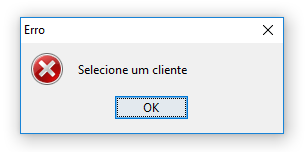
\includegraphics[]{erroencomenda.png}
	\caption{Erro - Cliente não selecionado}
	\label{erroencomenda}
\end{figure}

\begin{figure}[H]
	\centering
	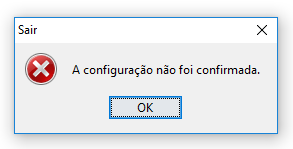
\includegraphics[]{erroencomenda2.png}
	\caption{Erro - Não confirma encomenda}
	\label{erroencomenda2}
\end{figure}



\subsubsection{Consultar clientes}
Para além da funcionalidade descrita na secção anterior, o \textit{Funcionário de loja} pode ainda, na janela apresentada na Figura \ref{clientesframe}, consultar, pesquisar e alterar clientes, assim como adicionar novos. 

Na tabela estão presentes os clientes registados no sistema até ao momento. Estes podem ser pesquisados pelo seu nome, utilizando para tal a caixa de texto presente debaixo da tabela. Ao fazer \textit{double click} sobre um cliente, é possível ver as suas características, bem como editar algumas delas (este processo é detalhado na secção \ref{alterarcliente}). Por fim, a partir desta janela é ainda possível a criação de novos clientes através do botão \textit{"Adicionar Cliente"} (como é demonstrado na secção \ref{novocliente}).

\begin{figure}[H]
	\centering
	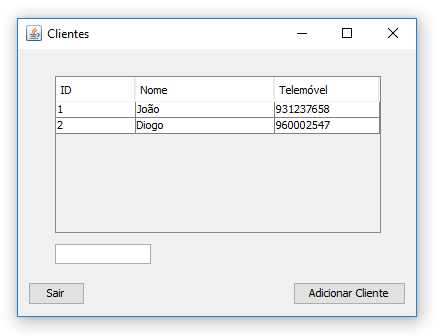
\includegraphics[]{clientesframe.png}
	\caption{Clientes Frame}
	\label{clientesframe}
\end{figure}


\myparagraph{Novo Cliente}
\label{novocliente} 

Para registar um novo cliente é necessário introduzir o seu nome, telemóvel e e-mail nas respestivas caixas de texto apresentadas na Figura \ref{novoclienteframe}.

\begin{figure}[H]
	\centering
	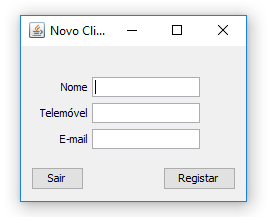
\includegraphics[]{novoclienteframe.png}
	\caption{Novo Cliente Frame}
	\label{novoclienteframe}
\end{figure}


\myparagraph{Alterar Cliente}
\label{alterarcliente}

Em relação à alteração de um cliente, apenas é permitido alterar o seu telemóvel e o seu e-mail. Para isso, é necessário que sejam feitas alterações nos respetivos campos, confirmando-as clicando em \textit{"Atualizar"}.

\begin{figure}[H]
	\centering
	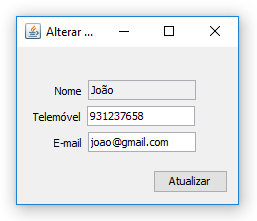
\includegraphics[]{alterarclienteframe.png}
	\caption{Alterar Cliente Frame}
	\label{alterarclienteframe}
\end{figure}


\subsection{Fábrica}
\label{fabricasec}

Quando a sessão é iniciada por um \textit{Gestor de Fábrica}, a janela correspondente é a seguinte:

\begin{figure}[H]
	\centering
	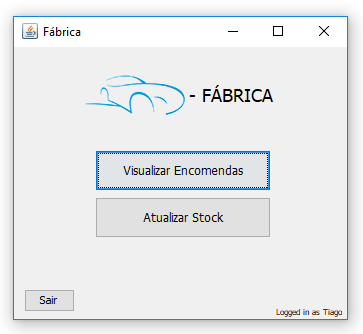
\includegraphics[]{fabricaframe.png}
	\caption{Fabrica Frame}
	\label{fabricaframe}
\end{figure}

Aqui, o funcionário pode visualizar as encomendas pendentes ou atualizar o stock da fábrica. Para isso, basta clicar nos botões \textit{"Visualizar Encomendas"} e \textit{"Atualizar Stock"}, respetivamente.

\subsubsection{Encomendas Pendentes}
A partir desta janela, o funcionário pode visualizar todas as encomendas pendentes. Além do mais, é ainda possível visualizar o seu conteúdo, selecionando a desejada e em seguida clicar em \textit{Consultar} ou então produzir, no botão \textit{"Produzir Encomenda}.

\begin{figure}[H]
	\centering
	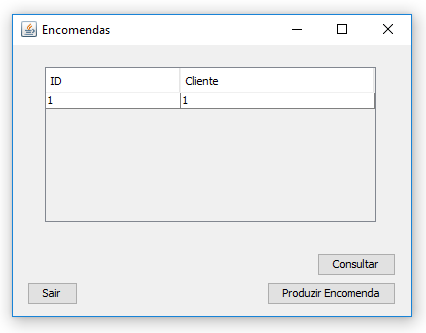
\includegraphics[]{encomendasframe.png}
	\caption{Encomendas Frame}
	\label{encomendasframe}
\end{figure}


\myparagraph{Consultar Encomenda}

Na Figura \ref{dencomendasframe}, é apresentado um exemplo dos detalhes de uma encomenda:

\begin{figure}[H]
	\centering
	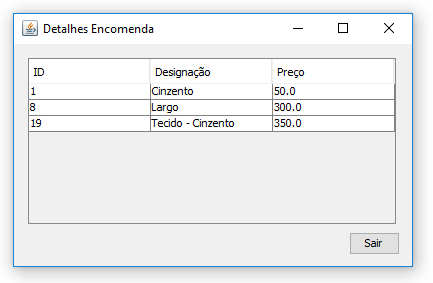
\includegraphics[]{detalhesencomenda.png}
	\caption{Detalhes Encomenda Frame}
	\label{dencomendasframe}
\end{figure}

\myparagraph{Produzir Encomenda}

Para que seja possível produzir uma encomenda, é necessário que exista stock de todas as componentes presentes na mesma. Uma possível mensagem é a seguinte:

\begin{figure}[H]
	\centering
	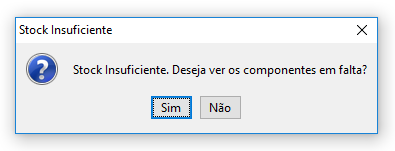
\includegraphics[]{stockinsuficiente.png}
\end{figure}

O utilizador ao responder "sim" são-lhe apresentadas, então, as componentes sem stock de momento:

\begin{figure}[H]
	\centering
	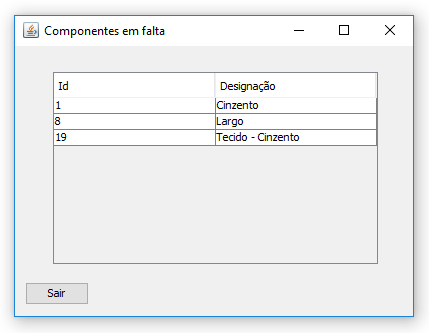
\includegraphics[]{componentesemfalta.png}
\end{figure}

\subsubsection{Stock}
Como se pode ver pela Figura \ref{stockframe}, nesta janela é apresentado todo o stock das componentes existentes (ordenado por ordem decrescente de stock). Para atualizar stock é necessário clicar em \textit{"Atualizar Stock"}. Esse processo é explicado na secção seguinte.

\begin{figure}[H]
	\centering
	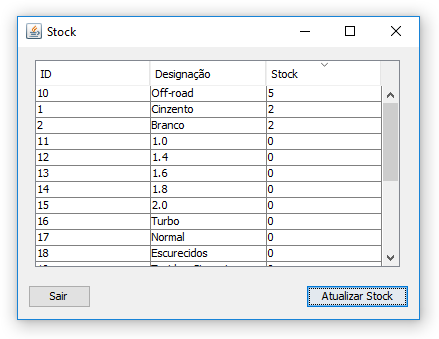
\includegraphics[]{stockframe.png}
	\caption{Stock Frame}
	\label{stockframe}
\end{figure}

\myparagraph{Atualizar Stock}

Quando o funcionário necessita de atualizar stock é confrontado com a seguinte janela:
\begin{figure}[H]
	\centering
	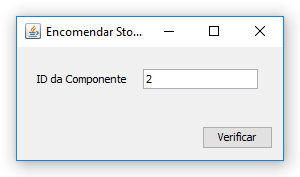
\includegraphics[]{encomendastock1.png}
\end{figure}

Caso o ID da componente introduzido exista prossegue introduzindo a quantidade:

\begin{figure}[H]
	\centering
	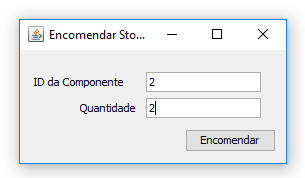
\includegraphics[]{encomendastock2.png}
\end{figure}

Caso não exista a componente o funcionário é interrogado se quer ou não adicionar nova componente:
\begin{figure}[H]
	\centering
	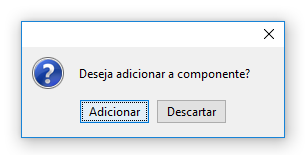
\includegraphics[]{adicionarcomp.png}
\end{figure}

Se não aceitar adicionar o processo para. Se adicionar tem então que introduzir as características da nova componente:
\begin{figure}[H]
	\centering
	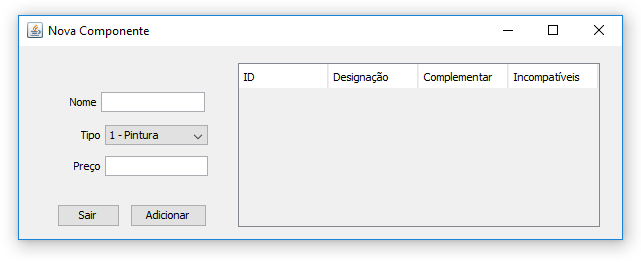
\includegraphics[width=5in]{novacomponente.png}
\end{figure}

Aqui é possível também adicionar componentes complementares ou incompatíveis caso existam algumas sem nenhum destes dois inconvenientes. Para finalizar este registo apenas tem que clicar em \textit{"Adicionar"}.


\subsection{Gestão de funcionários}
\label{adminsec}

Por fim, o último caso de login é quando ele é realizado pelo administrador. A partir da janela identificada na Figura \ref{funcionariosframe}, este é capaz de adicionar novos funcionários e gerir os já existentes. Para a primeira funcionalidade, o utilizador necessita de clicar no botão \textit{"Adicionar funcionário"} enquanto que para a segunda é necessário fazer \textit{double click} no funcionário desejado. Estas funcionalidades são explicadas mais detalhadamente nas secções em seguida (\ref{novofunc} e \ref{alterafunc}, respetivamente). É também possível para o utilizador pesquisar por um funcionário através da caixa de texto presente na janela. A tabela dos funcionários é atualizada conforme o que é introduzido nessa caixa.


\begin{figure}[H]
	\centering
	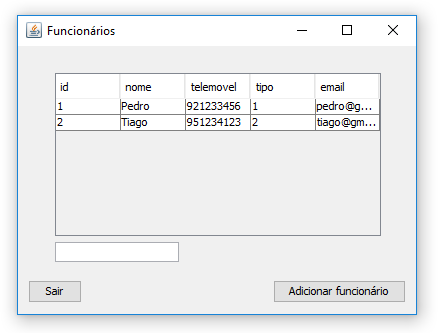
\includegraphics[]{funcionariosframe.png}
	\caption{Funcionarios Frame}
	\label{funcionariosframe}
\end{figure}

\subsubsection{Novo funcionário}
\label{novofunc}

Para a criação de um novo funcionário é necessário preencher todos os campos presentes na Figura \ref{novofuncframe}. O tipo do funcionário pode variar entre \textit{"1 - Funcionário de loja"} e \textit{"2 - Gestor de fábrica"}.

\begin{figure}[H]
	\centering
	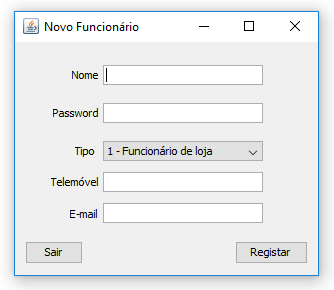
\includegraphics[]{novofuncframe.png}
	\caption{Novo Funcionário Frame}
	\label{novofuncframe}
\end{figure}


\subsubsection{Alterar funcionário}
\label{alterafunc}

Nesta janela, e para concluir a interface, é possível, como referido anteriormente, gerir o funcionário selecionado. Esta gestão pode ser a alteração dos seus dados (exceto \textit{nome} e \textit{password}) ou a sua remoção do sistema.

\begin{figure}[H]
	\centering
	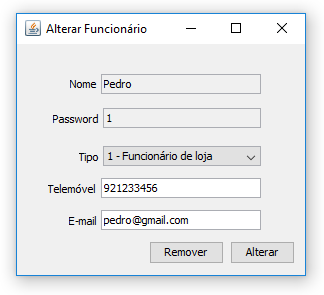
\includegraphics[]{alterarfuncframe.png}
	\caption{Alterar Funcionário Frame}
	\label{alterarfuncframe}
\end{figure}
\newpage